% =====================================================================
% report_additions.tex
% Ready-to-paste LaTeX for updating report.pdf with the fixes.
% All numbers come from the regenerated pipeline (data/ directory).
%
% Requires these packages in your preamble (add any that are missing):
%   \usepackage{booktabs}   % for the results table
%   \usepackage{graphicx}   % for the figures
% =====================================================================


% ---------------------------------------------------------------------
% (A) DATA SPLITTING / METHODOLOGY  -- paste into the Methods section,
%     replacing the current description of the train/test split.
% ---------------------------------------------------------------------
Sequences were first made non-redundant with MMseqs2 (30\% sequence
identity, 40\% coverage) over the \emph{complete} positive and negative
sets, so that no homologous pair can be split between training and test.
The retained cluster representatives were then shuffled with a fixed
random seed (42) and partitioned 80/20 into a training and a held-out
test set; the training set was further divided into five equal folds for
cross-validation. For the von Heijne model, the position-specific weight
matrix and its decision threshold are selected jointly from the single
fold with the highest validation F1, ensuring that the chosen matrix and
threshold originate from the same fold.


% ---------------------------------------------------------------------
% (B) BIOCHEMICAL FEATURES  -- paste into the feature/results discussion.
% ---------------------------------------------------------------------
Averaged over the five cross-validation folds, the Random-Forest Gini
importances are dominated by hydrophobicity and closely related
properties: \texttt{max\_hydrophobicity} (0.092), \texttt{tm\_position}
(0.065), \texttt{max\_aliphacity} (0.061) and \texttt{mean\_hydrophobicity}
(0.057), with the ten most important features accounting for roughly
51\% of the total importance and the ranking remaining stable across
folds. This matches the biology of the problem, where the discriminative
signal is the hydrophobic h-region of the signal peptide, and explains
why charge and secondary-structure descriptors contribute comparatively
little; it also motivates the feature-selection step, since a small
hydrophobicity/aliphacity/transmembrane-propensity core carries most of
the signal.


% ---------------------------------------------------------------------
% (C) KINGDOM / SPECIES ANALYSIS  -- paste into the exploratory section.
% ---------------------------------------------------------------------
The dataset is imbalanced, with 7.1 negatives per positive (2{,}960 vs
20{,}944), and the two classes differ taxonomically: positives are
dominated by Metazoa (82.6\%), whereas negatives are spread across
Metazoa (60.2\%), Viridiplantae (19.7\%) and Fungi (18.2\%). At the
species level \emph{Homo sapiens} alone provides 25\% of the positives
and 30\% of the negatives, with the negative set further concentrated in
a few model organisms (mouse, \emph{Arabidopsis}, \emph{S.\ cerevisiae}).
This is relevant for interpretation: the model is trained predominantly
on animal signal peptides, so its behaviour on plant and fungal signal
peptides is effectively extrapolation and the reported metrics may not
transfer uniformly across kingdoms. Positives are also markedly shorter
(median 214 vs 436 residues), although only the first 40--90 residues
enter the features, so this length difference does not directly bias the
classifier.


% ---------------------------------------------------------------------
% (D) FALSE-POSITIVE / TRANSMEMBRANE ANALYSIS  -- paste into the error
%     discussion.
% ---------------------------------------------------------------------
Transmembrane proteins make up 12.1\% of the negative set, but are
strongly over-represented among the false positives. The von Heijne
model produces 86 false positives, 57\% of which are transmembrane --- a
4.7$\times$ enrichment over the base rate --- confirming that a
hydrophobic transmembrane helix is readily mistaken for a cleavable
h-region by a purely hydrophobicity-based PSWM. The SVM, which receives
explicit transmembrane-propensity and positional features, both reduces
the false positives to 25 ($-71\%$) and lowers their transmembrane
fraction to 44\% (3.6$\times$ enrichment). The biochemical features
therefore partially resolve the main confounder, although the residual
44\% shows that the signal-peptide / transmembrane distinction is not
fully solved.


% ---------------------------------------------------------------------
% (E) RESULTS TABLE  -- paste where you compare the models.
% ---------------------------------------------------------------------
\begin{table}[ht]
\centering
\begin{tabular}{lccccc}
\toprule
Model & Accuracy & Precision & Recall & F1 & MCC \\
\midrule
von Heijne PSWM         & 0.933 & 0.665 & 0.774 & 0.715 & 0.680 \\
SVM (all features)      & 0.971 & 0.889 & 0.833 & 0.860 & 0.844 \\
SVM (selected features) & 0.970 & 0.880 & 0.833 & 0.856 & 0.839 \\
FFNN                    & 0.962 & 0.798 & 0.873 & 0.834 & 0.813 \\
\bottomrule
\end{tabular}
\caption{Test-set performance of the von Heijne baseline, the SVM models
and the feed-forward neural network (221 positives, 1{,}816 negatives).}
\label{tab:results}
\end{table}


% ---------------------------------------------------------------------
% (F) FEED-FORWARD NEURAL NETWORK  -- new subsection for the Advanced
%     module. Place it after the SVM section.
% ---------------------------------------------------------------------
\subsection{Feed-forward neural network}

A feed-forward neural network was trained on the same 39 biochemical
features used by the SVM. A small architecture search (one or two hidden
layers) was evaluated by five-fold cross-validation on the same folds and
selected by mean validation MCC, yielding a single hidden layer of 64
ReLU units trained with Adam (learning rate $10^{-3}$, $L_2$
regularisation $\alpha=10^{-3}$, batch size 64, up to 400 epochs) on
standardised features. The class imbalance ($\approx$8:1) was handled by
seeded oversampling of the minority class during training and by tuning
the decision threshold for maximum MCC on the pooled out-of-fold
predictions (so the test set is never used for threshold selection). On
the held-out test set the network reached MCC 0.813 and F1 0.834
(accuracy 0.962, precision 0.798, recall 0.873), comparable to the SVM
(MCC 0.839) and with the highest recall of all models. Training curves
for the selected architecture are shown in
Figure~\ref{fig:ffnn_curves}, and the confusion matrix in
Figure~\ref{fig:ffnn_cm}.

\begin{figure}[ht]
\centering
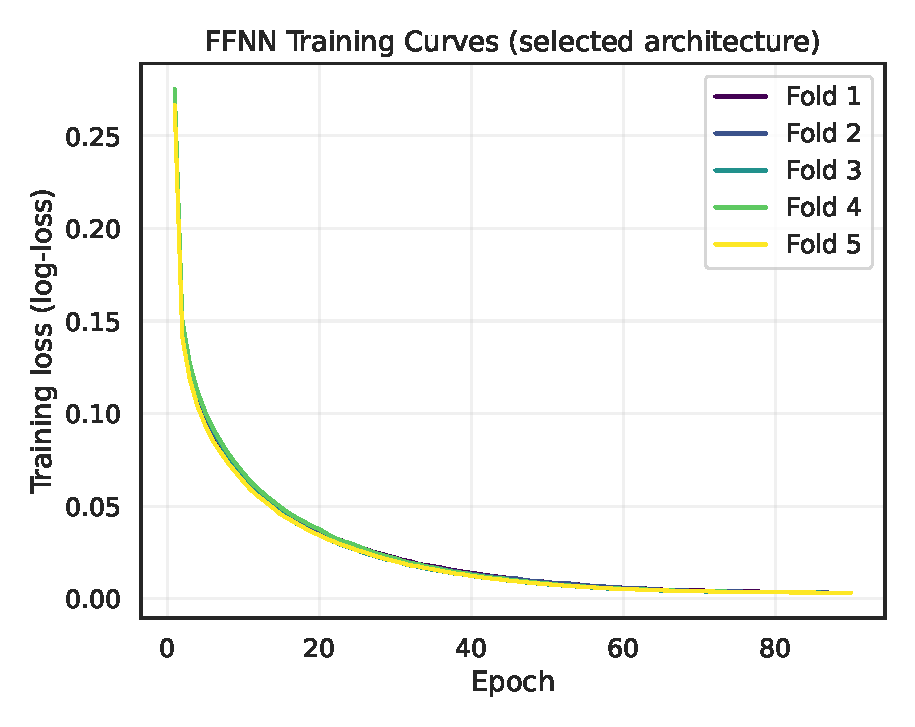
\includegraphics[width=0.7\linewidth]{data/ffnn/training_curves.pdf}
\caption{FFNN training loss per epoch across the five cross-validation
folds (selected architecture).}
\label{fig:ffnn_curves}
\end{figure}

\begin{figure}[ht]
\centering
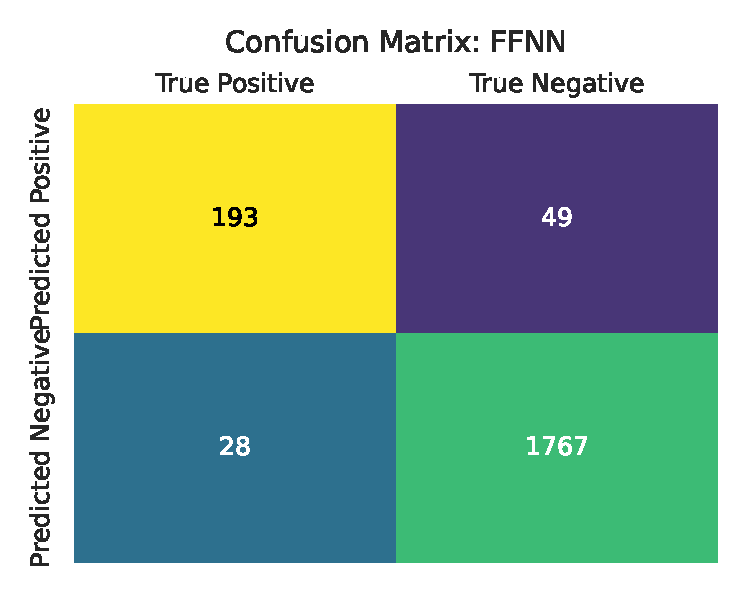
\includegraphics[width=0.5\linewidth]{data/ffnn/confusion_matrix.pdf}
\caption{Confusion matrix of the FFNN on the held-out test set.}
\label{fig:ffnn_cm}
\end{figure}
